\newcommand\SCALE{0.8}

\section{Experimentation}
\label{sec:experimentation}


In this section, we evaluate how the adaptiveness of \SPRAY impacts common
metrics of peer-sampling performance including clustering coefficient, average
shortest path length, in-degree distribution, robustness, and arc count. We
compare \SPRAY with a representative of fixed-size partial view approaches,
namely \CYCLON. We expect \SPRAY and \CYCLON to exhibit similar behaviors when
\CYCLON is optimally configured in advance to handle the network size. We expect
\SPRAY to save resources when \CYCLON is oversized, and to be more robust when
\CYCLON is undersized. Finally, we expect \SPRAY to keep a negligible number of
duplicates in its partial views. We also evaluate the impact of the WebRTC
connection establishment on \CYCLON, \SCAMP, and \SPRAY, in networks subject to
message loss.  We expect a normal behavior for \CYCLON and \SPRAY while \SCAMP
becomes quickly partitioned.

The experiments run on the \PEERSIM simulator~\cite{montresor2009peersim}, a
well-known program written in Java that allows simulations to reach high scale
in terms of number of peers. Our implementation of the evaluated random peer
sampling protocols is available on the Github
platform\footnote{\url{https://github.com/justayak/peersim-spray}}.


\subsection{Clustering and convergence time}

\begin{asparadesc}
\item[Objective:] To observe how adaptiveness impacts clustering and convergence
  time.
\item[Description:] The average local clustering
  coefficient~\cite{watts1998collective} measures peers' neighborhood
  connectivity in the network:
  \begin{equation*}
    \overline{C} = {1\over |V^t|}\sum\limits_{x\in V^t}C_x
  \end{equation*}
  where $C_x$ is the local clustering coefficient of Peer $p_x$. The higher the
  coefficient, the more peers are tied together. The coefficient of complete
  graphs is 1. The coefficient of random graphs is close to 0.  

  For each approach, the experiment comprises 4 runs respectively building a
  network of 0.1k, 1k, 10k, and 100k peers. Peers join the network at
  once. Peers join the network through a contact peer chosen at random following
  a uniform distribution. The representative of the fixed-size approach is
  \CYCLON which is optimally configured for 1k peers: $\ln(1000)\approx 7$
  neighbors.  \CYCLON is oversized for 0.1k peers and undersized for 10k peers
  and 100k peers. During exchanges, the peers using \CYCLON shuffle $3$ out of
  their $7$ neighbors.

\begin{figure}
  \centering
  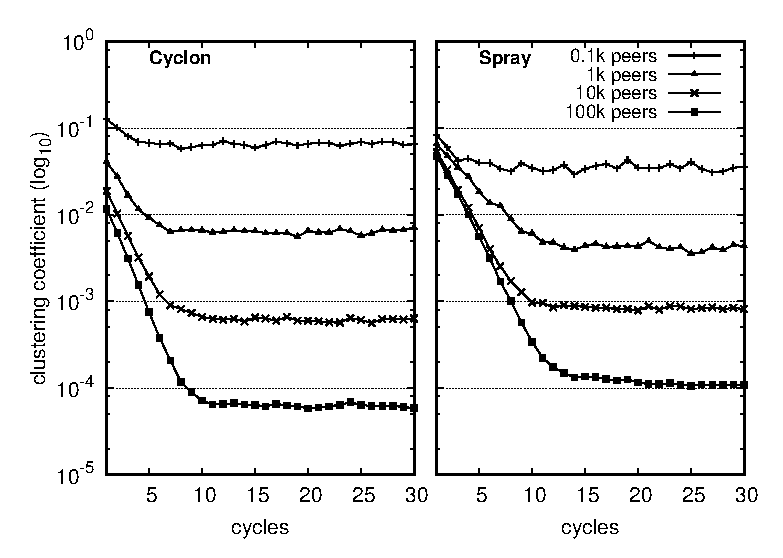
\includegraphics[width=\SCALE\textwidth]{img/clustering.eps}
  \caption{\label{fig:clustering}Clustering coefficient.}
\end{figure}

\item[Results:] Figure~\ref{fig:clustering} shows that \CYCLON starts with a
  lower clustering coefficient than \SPRAY.  Yet, \CYCLON and \SPRAY have
  roughly similar convergence time, for it converges exponentially fast.
  Figure~\ref{fig:clustering} also shows that both approaches converge to a low
  clustering coefficient which is characteristic of random graphs. Nevertheless,
  \CYCLON and \SPRAY do not reach the same values after convergence. Except when
  \CYCLON's configuration aims for 1k peers, \SPRAY's values are either below
  (when \CYCLON is oversized) or above (when \CYCLON is undersized).
  
  These results show that both \SPRAY and \CYCLON can be deployed at once. They
  start ready-to-use but do not have their optimal properties. However, no
  matter the size of the deployment, they will obtain these properties very
  quickly.

\item[Reasons:] Peers join one after the other in 1 round. Peers join using a
  contact peer chosen at random among already connected peers. Therefore, old
  peers are chosen more often during this starting round. In the starting
  topology, old peers are more clustered than newest ones. In particular, since
  \SPRAY does not enforce a limit on the size of partial views, oldest peers
  have larger partial views than newest peers. Thus, oldest peers are more tied
  together. Consequently, \SPRAY starts with a higher clustering coefficient
  than \CYCLON. 

  The clustering coefficient measures how much peer's neighbors are connected
  together. It directly depends on the partial view size of each peer which, in
  \CYCLON, is constant. Thus, when the number of peers is multiplied by $10$,
  the clustering coefficient after convergence is divided by $10$. On the other
  hand, peers using \SPRAY have a partial view the size of which reflects the
  network size. When the network has 1k peers, \SPRAY and \CYCLON have roughly
  the same average partial view size (\SPRAY $7.1$ vs \CYCLON $7$), hence almost
  identical clustering coefficient measurements. By extending the reasoning,
  this also explains why \SPRAY yields lower $\overline{C}$ values when \CYCLON
  is oversized, and why it yields higher values when \CYCLON is undersized.
\end{asparadesc}


\subsection{Information dissemination}

\begin{asparadesc}
\item[Objective:] To observe how adaptiveness impacts the average shortest path
  length, i.e., the speed of information dissemination.
\item[Description:] The average path length is the average of the shortest path
  length between peers in the graph. It counts the minimum number of hops to
  reach a peer from another given peer. It basically represents the traveling
  time of any information to reach all the peers at least once. We average the
  path length on a subset of the network membership.

  We run the simulation on \SPRAY $100$ times to avoid any side effects due to
  randomness. The experiment comprises 3 runs for \CYCLON: \CYCLON set to 7
  neighbors targets 1k peers; \CYCLON set to 9 neighbors targets 8k peers;
  \CYCLON set to 11 neighbors targets 60k peers. We perform the measurements
  after convergence. The checkpoints for the measurements are 0.1k, 0.5k, 1k,
  5k, 10k, 50k, and 100k peers.

\begin{figure}
  \centering
  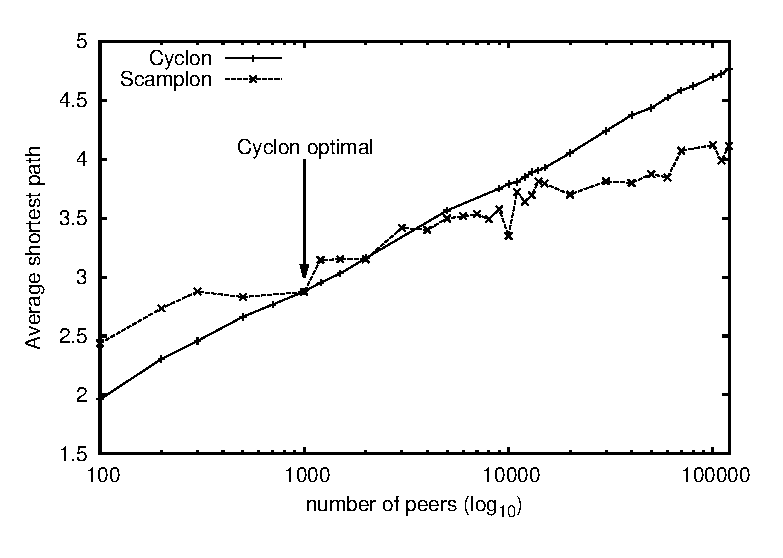
\includegraphics[width=\SCALE\textwidth]{img/avgpath.eps}
  \caption{\label{fig:avgpath}Average shortest path length.}
\end{figure}

\item[Results:] Figure~\ref{fig:avgpath} shows that both \CYCLON and \SPRAY have
  a relatively small average shortest path length.  Figure~\ref{fig:avgpath}
  also shows that each run of \CYCLON is divided in three parts compared to
  \SPRAY. First, an oversized \CYCLON has smaller values than \SPRAY. Then,
  \SPRAY and \CYCLON become equivalent where the latter is optimally
  configured. Finally, \SPRAY has smaller values than \CYCLON. Overall, \SPRAY
  scales better than \CYCLON since the gradient (slope) of the former is lower
  than any configuration of the latter.

  These results show that developers could use both \SPRAY and \CYCLON to build
  efficient information dissemination protocols. Nevertheless, they should use
  \SPRAY over \CYCLON if their concerns are about latency and the network size
  is unknown or can change over time.

\item[Reasons:] We performed the measurements after convergence. After
  convergence, the network overlay become closely related to random graphs. In
  particular, the diameter and average shortest path length remain small.

  Since the number of arcs using an oversized \CYCLON is greater, it yields a
  lower average path length than \SPRAY. Conversely, since the number of arcs
  using an undersized \CYCLON is lower, \SPRAY achieves better performance
  thanks to its larger partial views. Overall, \SPRAY scales better than any
  configuration of \CYCLON, for it adds arcs as the network grows.
\end{asparadesc}


% \begin{figure*}
%   \centering
%   \subfloat[Figure A][\label{fig:churnA}Global number of arcs during an experiment 
%   including churn.]{
%     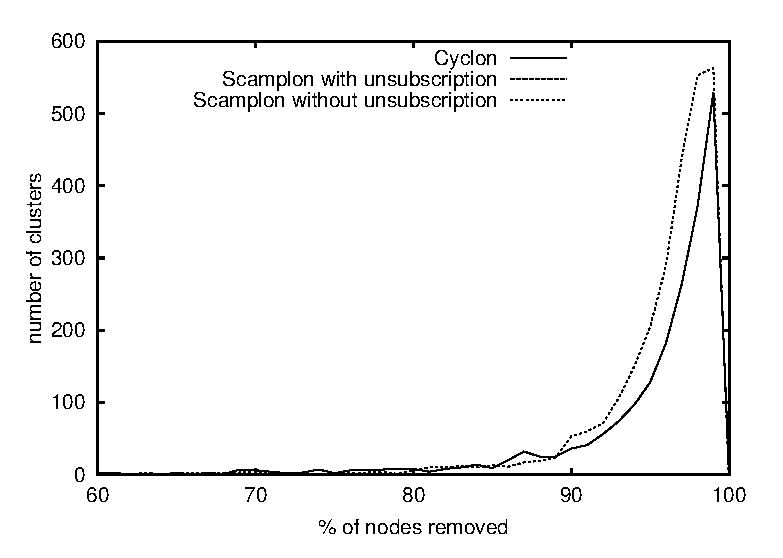
\includegraphics[width=0.48\textwidth]{img/churn.eps}}
%   \hspace{10pt}
%   \subfloat[Figure B][\label{fig:churnB}Average partial view size during an experiment
%   including churn.]{
%     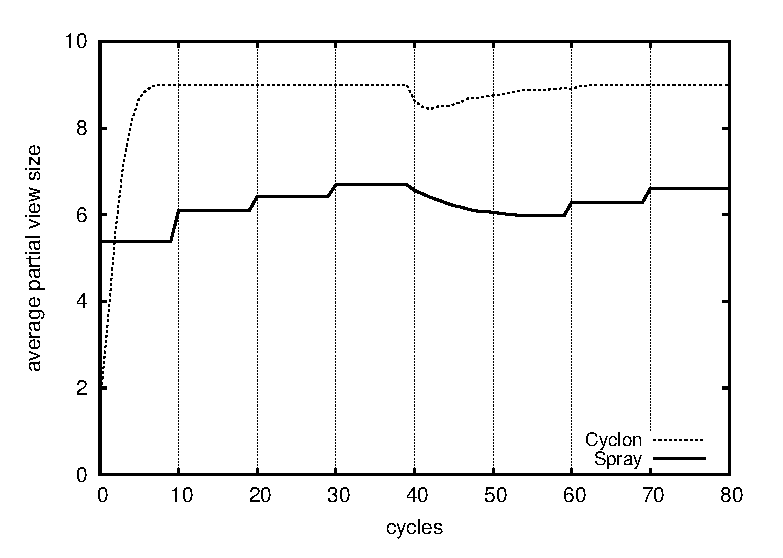
\includegraphics[width=0.48\textwidth]{img/avgpv.eps}}
% \end{figure*}

\subsection{Load-balancing}

\begin{asparadesc}
\item[Objective:] To observe how adaptiveness impacts the in-degree
  distribution, i.e., the load-balancing among peers.
\item[Description:] The in-degree of a peer shows how well it is represented in
  others' partial views. The in-degree distribution of the network can highlight
  the existence of weakly connected peers and strongly connected hubs. These
  peers have an in-degree far from the average in-degree value. It directly
  impacts robustness, for few crashes or departures may disconnect a weakly
  connected peer; and disconnections of hubs deeply impact the rest of the
  network.

  For each approach, the experiment comprises 4 runs respectively building a
  network of 0.1k, 1k, 100k, and 500k peers. We configure \CYCLON with partial
  views of size $7$ which targets a network of 1k peers.  We perform the
  in-degree measurements after convergence.

\begin{figure}
  \centering
  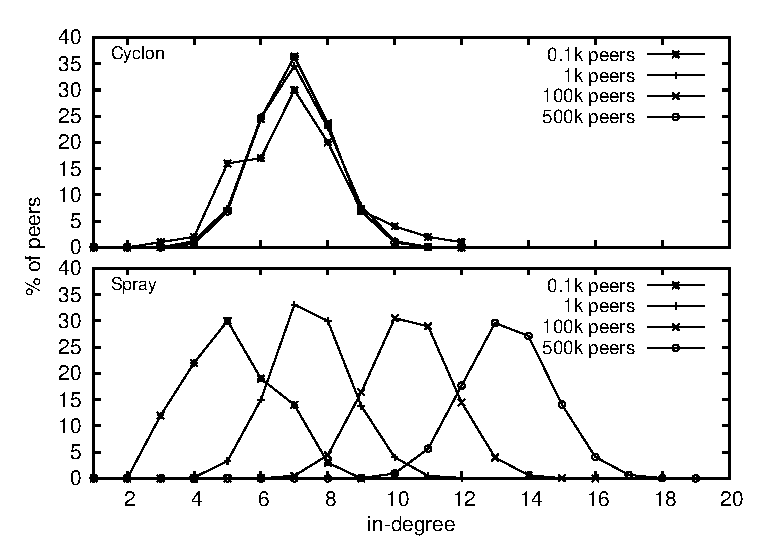
\includegraphics[width=\SCALE\textwidth]{img/histo.eps}
  \caption{\label{fig:histo}In-degree distribution.}
\end{figure}

\item[Results:] Figure~\ref{fig:histo} shows the in-degree distribution of
  \CYCLON and \SPRAY. The x-axis denotes the in-degree. The y-axis denotes the
  percentage of peers with such in-degree in the network. The top part of
  Figure~\ref{fig:histo} focuses on \CYCLON. We observe that the in-degree
  distributions are identical independently of the network size. For instance,
  the distribution of 0.1k peers is identical to the one of 500k peers. The mean
  value is roughly 7 and we observe a strong peak on this value. On the other
  hand, the bottom part of Figure~\ref{fig:histo} focuses on \SPRAY. We observe
  that the distribution of \SPRAY follows the average partial view size, which
  itself follows the growth of the size of the network.

  Figure~\ref{fig:histo} also shows that peers are very gathered around the mean
  partial view size for both \SPRAY and \CYCLON. For instance, for the run with
  500k peers using \SPRAY, the mean in-degree value is 13.37 and 88\% of peers
  have an in-degree between 12 and 14 included. Even the highest in-degree value
  18 is not far from the average in-degree. Thus, there are no weakly connected
  peers nor strongly connected hubs.

  These results show that both \SPRAY and \CYCLON are resilient to random
  failures, for peers are equally important in terms of connectedness. These
  results also show that developers could use both \SPRAY and \CYCLON to build
  dissemination protocols that would balance the download among peers. Using
  \SPRAY, the download would increase and decrease following the fluctuations in
  network size.

\item[Reasons:] Once configured, \CYCLON must handle any number of peers in the
  network with a fixed-size partial view and since the partial view size is
  constant, the in-degree of peers stays stable.  On the other hand, in \SPRAY,
  each joining peer brings an increasing number of arcs in the network. Thus,
  the in-degree of peers slowly grows reflecting the network size. Hence, the
  distribution in the bottom part of Figure~\ref{fig:histo} shifts slowly to
  higher in-degree values as the network size grows.

  \SPRAY does not peak on a particular value as \CYCLON does because the average
  partial view size for a particular network size may fall in-between integer
  values. For instance, if peers using \SPRAY have partial views that contain
  6.5 neighbors on average, it means that half these peers have 6 neighbors
  while the other half have 7 (out-degree). As consequence, the average
  in-degree value will also be 6.5. However, while \SPRAY and \CYCLON constrain
  the size of partial views respectively to the average and to a constant value,
  they do not constrain the size of in-views, hence the distributions of
  Figure~\ref{fig:histo}.
\end{asparadesc}


\subsection{Adaptive partial views}

\begin{figure*}
\centering
\subfloat[Figure A]
[\label{fig:small}Mininum, maximum, average, and standard deviation of
the size of partial views.]
{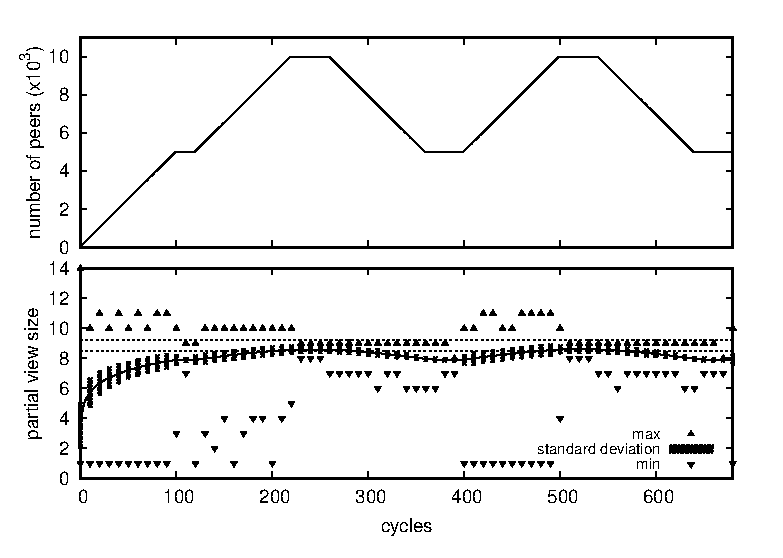
\includegraphics[width=0.8\textwidth]{img/small.eps}}

\subfloat[Figure B]
[\label{fig:extended}Average size of partial views over long period of time.]
{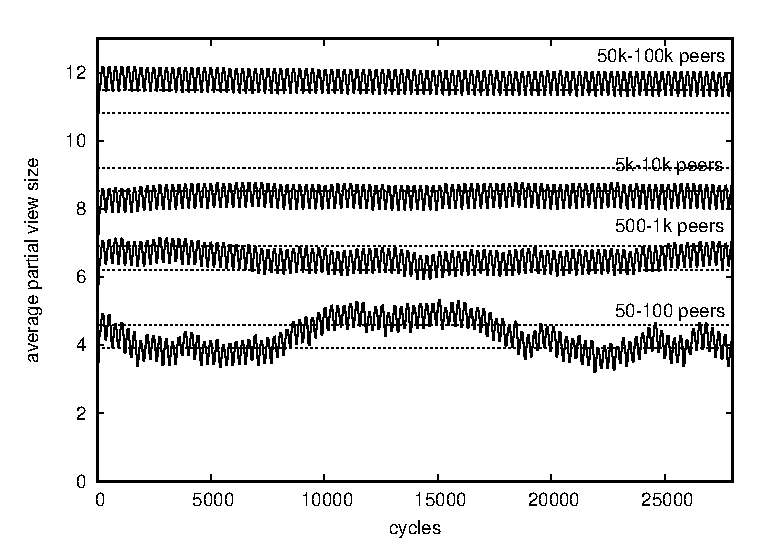
\includegraphics[width=0.8\textwidth]{img/extended.eps}}%
\caption{Partial view size measurements in networks subject to churn.}
\end{figure*}

\begin{asparadesc}
\item [Objective:] To show that using \SPRAY, the partial views grow and shrink
  logarithmically compared to the network size.
  %% To show that \SPRAY is non-deterministic
\item [Description:] In this experiment we focus on dynamic networks where peers
  can join and leave. In this experiment, we create 4 networks that vary from 50
  to 100 peers, from 500 to 1k peers, from 5k to 10k peers, and 50k to 100k
  peers. First, we create a network of half the maximum targeted size. Second,
  we repeatedly inject then disconnect half the maximum targeted size in periods
  of 240 cycles including a 40 cycles break in between injection and
  disconnection phases. For instance, in the network the size of which varies
  from 50k to 100k, 500 peers join the network at each cycle during the
  injection phases until it reaches 100k peers; then 40 cycles last; then 500
  peers leave the network at each cycle during the disconnection phases until it
  reaches 50k peers, and so on. During the experiments, we measure the maximum,
  the minimum, the average, and the standard deviation of the size of partial
  views.
\item [Results:] Figure~\ref{fig:small} focuses on the first 680 rounds of the
  experiment about the network varying from 5k to 10k peers. The top part of the
  figure shows the number of peer over time. The bottom part of the figure shows
  the measurements made on partial views. We observe that 
  \begin{inparaenum}[(i)]
    \item partial views grow logarithmically when the network size increases;
    \item partial views shrink logarithmically when the network size shrinks;
    \item while the extreme values of partial view size are spread during
      joining phases (from 1 to 12), standard deviation remains small, meaning
      that most of peers have the same partial view size.
  \end{inparaenum}
  Figure~\ref{fig:extended} shows the results of the 4 runs over 28k cycles,
  i.e., 100 injection/removal phases. The x-axis denotes the time in cycles. The
  y-axis denotes the average partial view size of peers. We observe
  that 
  \begin{inparaenum}[(i)]
  \item the average partial view size does not necessarily fit exactly the theoretical
    expectation;
  \item the average partial view size varies even for a network reaching the
    same number of peers;
  \item variations are more important as the number of peers is lower.
  \end{inparaenum}

  These results show that developers could use \SPRAY to deploy protocols such
  as distributed hash tables~\cite{camarillo2014self} or routing
  protocols~\cite{kleinberg2000smallworld} that normally require the use of
  network size estimators to work. The estimate provided by \SPRAY is not
  precise but comes at no cost while network size estimators involve traffic.

\item [Reasons:] A peer joining the network injects at least one arc plus a
  number of arcs depending on the contact peer. Since we choose the contact peer
  at random, and the partial views are averaged over shuffles, this number of
  injected arcs is the average partial view size on average. It leads to a
  logarithmic progression of the number of arcs. However, the peer joining the
  network only have one peer in its partial view while adding more arcs to its
  contact's neighborhood. Since we choose the contact peer at random, it may be
  chosen multiple times during 1 cycle which increases quickly its neighbors'
  number of arcs above the average. Consequently, we observe a large difference
  between the minimum and the maximum, but the standard deviation remains
  low. The latter is even more lowered after shuffling, for it makes partial
  views converge to their average size. 

  When a peer leaves the network, there is a logarithmic number of peers that
  detect the departure. They probabilistically duplicate an arc in such manner
  that one of them do not. Overall, it removes a logarithmic number of arcs plus
  one which correspond to the number of arcs injected during the latest
  joining. Consequently, the partial views shrink logarithmically when the
  network size diminishes.

  If we choose multiple time a same contact peer, its neighbors' number of arcs
  increases above the average. If one of these neighbors is chosen as contact
  peer before any shufflings, the global number of arcs increases too
  quickly. On the other hand, we may choose the newest peers as contact node
  hence increasing the number of arc too slowly, for they have fewer
  neighbors. Depending on these choices, the average partial view size can grow
  too high or too low compared to the theoretical value. Yet, it remains
  logarithmic, for these choices are made at random following a uniform
  distribution. These choices are more influential when the network size is low,
  for any addition or removal of arcs is proportionally more important.
\end{asparadesc}

% \subsection{Adaptive partial view}

% \begin{asparadesc}

% \item[Objective:] To show the impact of adaptiveness over partial view size when
%   the network size grows and shrinks over time.
% \item[Description:] In this experiment we focus on a dynamic network where peers
%   can join and leave.  \CYCLON's configuration targets 8k peers. It is
%   oversized compared the network size during the simulation (maximum of 1k
%   peers). During the first half of the experimentation, 250 peers are added 4
%   times successively by intervals of 10 cycles each. Thus, the network size goes
%   from 0 to 1k peers in 40 rounds. Then, half of the network leaves without
%   giving notice (500 peers). Finally, 250 peers join two additional times. The
%   final network contains 1k members. The measurements concern the average
%   partial view size.

% \begin{figure}
%   \centering
%   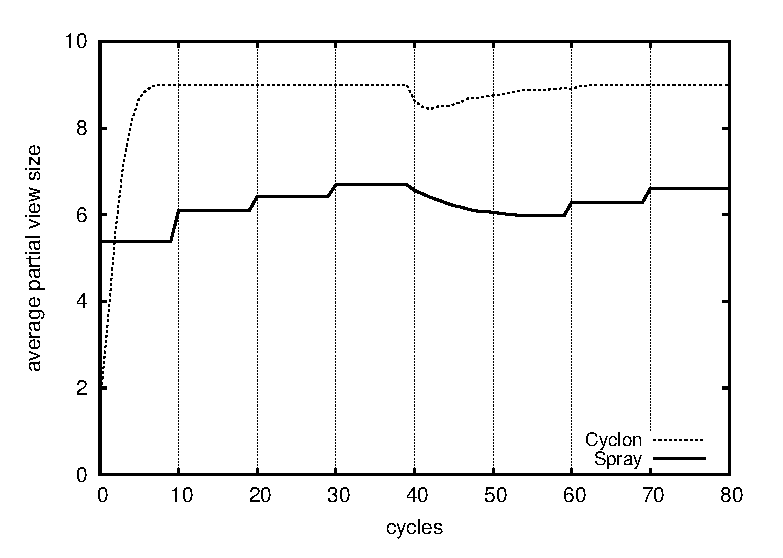
\includegraphics[width=\SCALE\textwidth]{img/avgpv.eps}
%   \caption{\label{fig:churn}Average partial view size with churn.}
% \end{figure}

% \item[Results:] Figure~\ref{fig:churn} shows the average partial view size of
%   \SPRAY and \CYCLON. As expected, \CYCLON immediately converges to the
%   configured partial view size (9 neighbors). On the other hand, \SPRAY's
%   partial views logarithmically grow while the network grows. When the removals
%   occur at cycle 40, the peers using \CYCLON remove the dead arcs while
%   refilling their partial view until they reach the configured partial view
%   size. The peers using \SPRAY only remove the arcs to reflect the departed
%   peers. At the end, the \SPRAY partial views contain on average 6.6 neighbors
%   (recall $\ln(1000)\approx 6.9$).
% \item[Reasons:] Since each peer injects a logarithmically growing number of
%   arcs, the average partial view size grows as more peers join the network.
%   The removal of 500 peers implies a decreasing slope. The slightly decreasing
%   number of arcs after the removal is due to peers realizing that some arcs are
%   dead, leading to a probabilistic removal (see Algorithm~\ref{algo:unreachable}).
% \end{asparadesc}


% \vspace{-7pt}
% \paragraph{Robustness}

\subsection{Robustness}

\begin{asparadesc}
\item[Objective:] To show \SPRAY's robustness to failures.
\item[Description:] To evaluate robustness, we count the number of weakly and
  strongly connected components of the network. Counting strong components
  allows us to estimate the effectiveness of information dissemination protocols
  built on top of random peer-sampling protocols. For example, with two strong
  components, bidirectional communication between the two components cannot be
  achieved. The first strong component may be able to reach the second, but the
  second may not reach the first. However, the network remains in a repairable
  state, for at least one link units these components. After some shuffling, the
  two strong components add links to each other. Thus, the two strong components
  merge into one. Therefore, counting the weak components allows us to estimate
  to what extent the network can be repaired, i.e., two weak components exist
  when there is no link to unit them.

  In our experiment, we configure \CYCLON's view size to 9, which targets 8k
  peers. The network contains 10k members. We perform the removals after the
  approaches have converged to a stable overlay network. We remove a random set
  of peers at once following a uniform distribution, from 25 to 95 percent of
  peers every 5 percents, i.e., 16 runs for each approach. We perform a last
  measurement at 99 percent. We measure the number of components immediately
  after each removal.

\begin{figure}
  \centering
  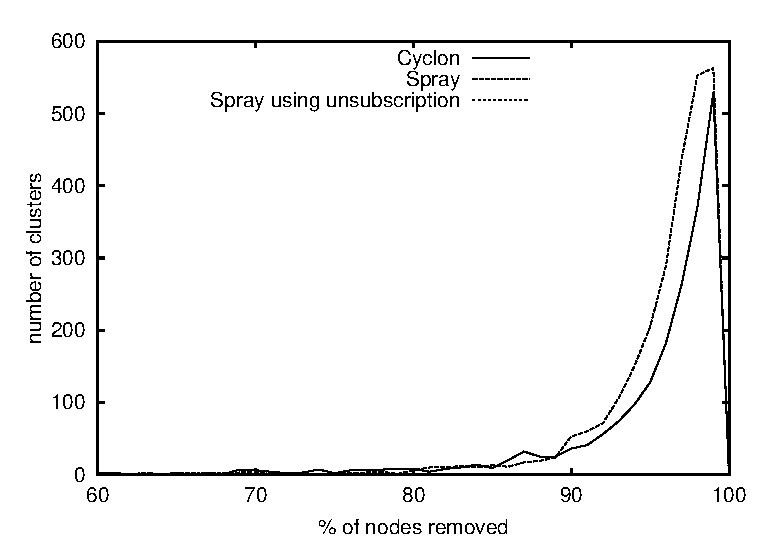
\includegraphics[width=\SCALE\textwidth]{img/resilience.eps}
  \caption{\label{fig:resilience}Robustness to massive failures.}
\end{figure}

\item[Results:] Figure~\ref{fig:resilience} shows the robustness of \SPRAY and
  \CYCLON to massive random failures. The x-axis denotes the percentage of peers
  removed at once. The y-axis denotes the ratio of strong/weak components over
  the network size after removals. First, Figure~\ref{fig:resilience} shows that
  both the random peer-sampling protocols \SPRAY and \CYCLON suffer from
  deteriorated behavior at high removal percentages, \CYCLON being slightly
  better in this term. Figure~\ref{fig:resilience} shows that the number of
  strong components starts to increase at 45 percents and to quickly increase at
  70 percents. Hence, the information dissemination starts to degrade at 45
  percents of removals: messages broadcast by some peers cannot reach all peers.
  Fortunately, Figure~\ref{fig:resilience} also shows that the approaches are
  able to recover from dire state until high removal ratio. Indeed, the number
  of weak components starts to increase at 70 percents of removals, meaning that
  there is no link between some parts of the network to unit them. In other
  terms, some parts of the network became completely disjoint. Shuffling cannot
  be initiated between members of each other disjoint parts. Consequently, the
  network cannot fully repair itself above 70 percents of removals.

  These results show that both \SPRAY and \CYCLON fit contexts such as the
  internet where numerous peers can join and leave freely in short periods of
  time.

  % Globally, Figure~\ref{fig:resilience} also demonstrates that the logarithmic
  % growth of these sampling protocols constitutes an upper bound, for
  % smaller growth could be obtained without endangering the connectedness of
  % the
  % network.
\item[Reasons:] The random peer-sampling approaches \CYCLON and \SPRAY yield
  very similar results because \CYCLON's configuration targets a network size of
  8k peers, while \SPRAY adjusts itself automatically to this network size.
  Therefore, the two protocols create very similar numbers of arcs. Yet \CYCLON
  performs slightly better for two reasons. First the variance in the degree
  distribution of \SPRAY causes \CYCLON to have more arcs in this specific
  experiment. Second, \SPRAY wastes some of its neighbors due to the presence of
  duplicate entries in its views (yet the number of duplicates remains small --
  see Figure~\ref{fig:duplicates}). Still both protocols preserve the ability to
  disseminate information until very large removal percentages. Another way to
  interpret this result consists in observing that when all peers have similar
  degrees, (see Figure~\ref{fig:histo}), removing a particular peer does not
  greatly affect connectedness. As suggested above, the direction of arcs
  impacts more information dissemination than the peer-sampling protocol
  itself. If an arc constitutes the last link between two clusters of the
  network, the messages from one of these clusters cannot reach the other
  one. Yet, this arc is enough for the peer-sampling protocol to start shuffling
  the views, ultimately populating them with members from both cluster. Hence,
  the network repairs itself.  When clusters become fully disjoints, neither
  \CYCLON nor \SPRAY is able to repair the network.

  % A smaller growth could be obtained because the sharp threshold of
  % connectedness applies to random graphs according to Erd{\H
  % o}s-R{\' e}nyi~\cite{erdos1959random}. However, random peer sampling
  % protocols constraint the partial views size to reduce the variance between
  % peers.  With such slight difference, we presume that a lower bound on arcs
  % growth could be found, although that may require global knowledge.
\end{asparadesc}

\subsection{Duplicates}

\begin{asparadesc} 
\item[Objective:] To show that a small proportion of peers contains duplicates
  in their partial view.
\item[Description:] Using \SPRAY as random peer-sampling protocol, we measure
  the amount of peers which have a partial view containing at least one
  duplicated reference. We perform the measurements on networks containing 0.1k,
  1k, 10k, 100k, and 500k peers. We measure the number of duplicates after
  convergence. We put this in relation with a theoretical approximation from the
  birthday paradox where the view size would be the number of randomly chosen
  people and the identity of peers would be the birthdates. The probability of a
  peer to \emph{not} have duplicates is approximately:
  \begin{equation*}
    1- 
    (1-
    \exp({-\ln(|V^t|)*(\ln(|V^t|)-1)\over{2*|V^t|}}))
  \end{equation*}

\begin{figure}
  \centering
  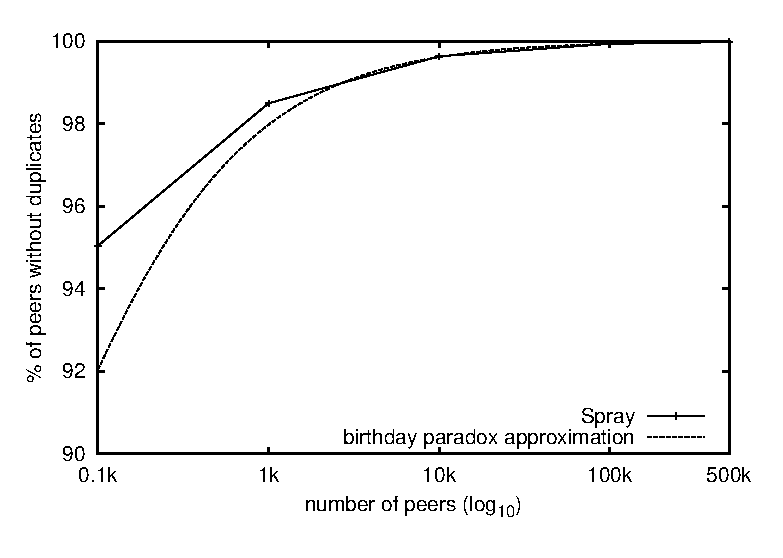
\includegraphics[width=\SCALE\textwidth]{img/duplicates.eps}
  \caption{\label{fig:duplicates}Duplicates in networks of different size.}
\end{figure}


\item[Results:] Figure~\ref{fig:duplicates} shows the proportion of peers using
  a partial view containing duplicates. We observe that there always exist
  partial views with at least one duplicate. The proportion is more important
  when the network size is small (e.g. 5 percents for 0.1k peers). It becomes a
  minor overhead when the network size is larger (e.g. less than 1 percent for
  10k peers). The birthday paradox approximation seems to follow very closely
  the experimental results. It empirically indicates that there exists a
  relation between the duplicates and the birthday paradox. The proportion of
  peers without duplicates tends to 100 percents as the network size grows.
\item[Reasons:] While the number of peers in the network grows linearly, the
  neighborhood size of each peer only grows logarithmically. This significant
  difference between the growths leads to the fact that the chances of a
  particular peer to have at least twice the reference to another peer becomes
  smaller as the number of peers in the network increases.
\end{asparadesc}


\subsection{Failures in connection establishment}
\label{subsec:degeneration}


\begin{asparadesc}
\item[Objective:] To show that \SPRAY does not suffer from failures in
  connection establishments, contrarily to \SCAMP.
\item[Description:] We measure both the arc count and the number of weak
  components in the network. The simulations involve \CYCLON (configured with
  partial view containing 9 neighbors targeting a network of roughly 8k
  peers), \SCAMP\footnote{A modified version of \SCAMP whose periodic protocol
    works properly when there is no connection failures. Available at
    \url{https://github.com/justayak/peersim-spray}}, and \SPRAY. They run over
  50k cycles. The network initially contains 10k members.  To establish a
  connection, we use the WebRTC three-way handshake, i.e., the initial peer
  emits an offer ticket, the arrival peer stamps the ticket, the initial peer
  finalizes the connection using the stamped ticket
  (see Section~\ref{sec:relatedwork}). The probability that the ticket fails to
  traverse a hop is set to $10^{-3}$.

\begin{figure}
  \centering 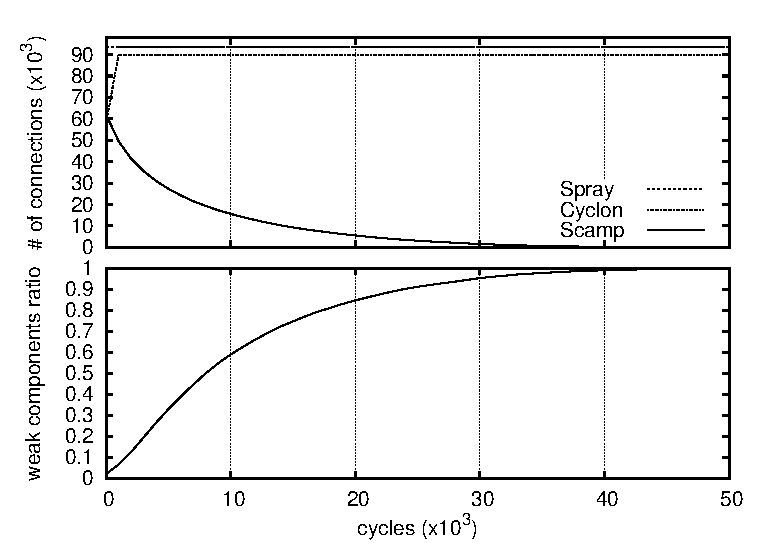
\includegraphics[width=\SCALE\textwidth]{img/degen.eps}
  \caption{\label{fig:degeneration}Number of arcs and partitioning in networks
    subject to failures in the connection establishments.}
\end{figure}

\item[Results:] The top part of Figure~\ref{fig:degeneration} shows the arc
  count of the random peer-sampling protocols while the bottom part of
  Figure~\ref{fig:degeneration} shows the weak components of the network.  As
  expected, we observe that the arc counts of \CYCLON and \SPRAY stays constant
  over cycles: 90k and 93k arcs for \CYCLON and \SPRAY respectively. On the
  other hand, \SCAMP suffers from failures in connection establishment. This
  directly impacts network connectedness as measured by the weak-component
  ratio. The network of \SCAMP quickly degrades.

  These results show that both \SPRAY and \CYCLON fit the constraints set by the
  connection establishement protocol of WebRTC.

\item[Reasons:] The arc counts of \CYCLON and \SPRAY remains constant
  over time but for different reasons. In \CYCLON, the shuffling
  protocol makes sure that the partial view is filled to its
  maximum. When a peer removes a broken connection, it replaces it
  with a fresh one in the following round.  In \SPRAY, when the
  protocol tries to use a broken connection, it replaces it with
  another known one. Thus, the arc count stays constant and the
  shuffling protocol makes sure that duplicates disappear over time
  (the arc moves to another peer where it is not a duplicate).
  \SCAMP, however, does not establish new connections with the
  neighbors of its neighbors.  Each hop of connection establishment
  process is an opportunity for failure.  Let $P_f$ be the probability
  that an element of the dissemination path (either a peer or a
  connection) crashes or leaves during a hop of the three-way
  handshake, without any possible recovery. Let $P_E$ be the
  probability that a connection establishment cannot be
  completed. Without three-way handshake, $P_E$ is straightforward:
  \begin{equation} P_{E,\,1way}^{Scamp}=1-(1-
    P_f)^{k+1} \end{equation} This corresponds to the probability that
  each element (arc and peer) in the path of size $k+1$ stays alive
  during the random walk. In the context of WebRTC, the offer ticket
  must travel back to its emitter. As a consequence, the elements of
  the random walk cannot fail until the stamped ticket travels
  back. We obtain:
  \begin{align} P_{E,\,3way}^{Scamp} &=1 - ((1-P_f)^{2(k+1)} (1-P_f)^{2k}
                                       \ldots (1-P_f)^2) \nonumber \\
                                     &=1-(1-P_f)^{k^2+3k+2}
  \end{align}
  In other terms, the first chosen arc and peer in the path must stay
  alive $2k+2$ hops, the second chosen arc and peer must stay alive
  $2k$ hops and so on.  This long duration leads to a quicker
  degeneration of the connection count.

  % This behavior endangers the network
  % connectedness.%%, as depicted in Section~\ref{subsec:degeneration}.

  % Since there is no routing in such network, the only way for a stamped ticket
  % to come back to its emitter is the path it traveled in the first place. Hence,
  % all peers belonging to the path must stay alive until the stamped ticket comes
  % back in order to consistently forward it.  Furthermore, its periodic protocol
  % starts with an immediate cutting of the incoming arcs of the initiating peer
  % because it assumes that each connection spread in the network will establish.
  % Since it does not, the peer eventually becomes disconnected. Also, when its
  % neighbors execute the periodic protocol, they delete their reference in its
  % partial view. In such case, the peer becomes disconnected and partitions
  % quickly appear.
\end{asparadesc}


%%% Local Variables:
%%% mode: latex
%%% TeX-master: "../paper"
%%% End:
